% #############################################################################
% This is Chapter 4 - Systematic Literature Review
% !TEX root = ../main.tex
% #############################################################################
% Carried over from the PIC report's Systematic Literature Review section.
% Adapted for the report class: headings promoted one level, figure paths
% rebased on ./Images/, every float given a unique label, and the article's
% hardcoded "Table N" references converted to \Cref so chapter-based
% numbering resolves correctly.
% #############################################################################
\fancychapter{Systematic Literature Review}
\label{chap:slr}

This chapter describes the execution of the systematic literature review, following the three SLR stages: Planning, Conducting, and Reporting the results.

\section{Planning the Review}

\subsection{Motivation}

AI, particularly LLMs and GenAI, is increasingly adopted across the SDLC to support code generation and completion, documentation, requirements engineering, automated bug fixing, and developer learning, and its use has been associated with productivity gains, improved efficiency, and support for complex development tasks \cite{Ahmed:2025ai, Zhang:2025ea, Durrani:2024ad, Jabrw:2025ss, Banh:2025cf, Farhanna:2025eu, KarlovsKarlovskis:2024ga, Terragni:2025fa}.

Adoption has nevertheless outpaced the resolution of the challenges it raises. The literature reports persistent concerns over the quality, reliability and trustworthiness of AI-generated artifacts, methodological barriers such as limited explainability and the black-box nature of advanced models, a heavy dependence on prompt formulation, and a concentration on isolated tasks that leaves several SDLC phases, particularly requirements engineering and design, with limited practical guidance.

\subsection{Research Questions}
Five research questions structure the review:

{\small
\begin{longtable}{p{0.7cm} p{7.5cm} p{6.5cm}}
\caption{Research Questions and Focus Areas}
\label{tab:RQs} \\
\toprule
\textbf{RQ} & \textbf{Research Question} & \textbf{Focus} \\
\midrule
\endfirsthead

\toprule
\textbf{RQ} & \textbf{Research Question} & \textbf{Focus} \\
\midrule
\endhead

\midrule
\multicolumn{3}{r}{\textit{Continued on next page}}\\
\bottomrule
\endfoot

\bottomrule
\endlastfoot

\textbf{RQ1} & What are the benefits of using and incorporating Vibe Coding, AI, and Large Language Models in software development? & Identify and categorize improvements in productivity, creativity, code quality, automation, collaboration, and innovation enabled by AI-driven tools. \\
\addlinespace

\textbf{RQ2} & What are the consequences that may arise from using and incorporating Vibe Coding, AI, and LLMs in software development, both in code generation and other sections? & Analyze risks such as technical debt, bias, reduced developer learning, code ownership, ethical issues, and dependency on AI tools. \\
\addlinespace

\textbf{RQ3} & What methodologies and management methods are being used to integrate Vibe Coding, AI, and LLMs into software engineering processes and workflows? & Explore frameworks, best practices, and process models (e.g., AI-augmented Agile, human-in-the-loop development, prompt engineering practices). \\
\addlinespace

\textbf{RQ4} & What are developers’ and other stakeholders’ opinions regarding the use of AI and LLMs in software development? & Assess perceptions, trust, satisfaction, and acceptance of AI-assisted coding among developers and organizations. \\
\addlinespace

\textbf{RQ5} & Which industry sectors are adopting AI for application development, and how do they benefit from its integration? & Map adoption trends across industries (e.g., finance, healthcare, IT, education), highlighting sector-specific motivations and outcomes. \\
\addlinespace

\end{longtable}}

\subsection{Review Protocol}
The criteria used for the literature search, stated in \Cref{tab:review_protocol}, returned 646 articles.

{\small
\centering

\begin{longtable}{p{2.8cm} p{12.2cm}}
\caption{Research Elements and Details}
\label{tab:review_protocol} \\
\toprule
\textbf{Element} & \textbf{Research Details} \\
\midrule
\endfirsthead

\toprule
\textbf{Element} & \textbf{Research Details} \\
\midrule
\endhead

\midrule
\multicolumn{2}{r}{\textit{Continued on next page}} \\
\bottomrule
\endfoot

\bottomrule
\endlastfoot

Source & EBSCO \\

\addlinespace
Final Search String &
(``Vibe Cod*'' OR ``AI models'' OR ``AI agen*'' OR ``large language model*'' OR ``generative AI'' OR openai OR ``chatgpt'' OR LLM* OR ``claude'' OR ``gemini'' OR copilot OR co-pilot) AND (``software development'' OR ``application development'' OR ``code generation'') \\
\addlinespace
Search Method & Search string found in the abstract of articles in English academic journals or conference materials, with no date range limit \\
\addlinespace
Results & 646 \\

\end{longtable}
}


"Vibe Coding" is the most recent term for the practice, but the practice predates the term, and querying it alone returned few relevant articles because the same work is published under different expressions. Synonymous keywords were added accordingly: it is the combination of "code generation" and "application development" with "generative AI" and "AI models" that retrieves the intended body of work, not any single term. The string was executed against the EBSCO Online Digital Library through its Advanced Search option, over the AB abstract field and the title, restricted to full-text-available results.

\section{Conducting the Review}

The second stage applies the filtering criteria to the 646 articles retrieved in the first; the attrition at each step is shown in \Cref{fig:article_filtering}.

\subsection{Filtering Process}

Extracting all 646 articles was not possible: EBSCO's page allows the download of 50 articles at a time, and after reloading and extending the page to its maximum the site displayed, in relevance order, only 467 of the 646.

The AI-powered systematic review management platform "Rayyan" was used to organise the articles. Of the 467 extracted, 117 duplicates were identified and removed, leaving 350 for abstract reading; that pass rejected 286 as belonging to a theme other than developing applications using AI, leaving 64 articles.

\begin{figure}[htbp]
     \centering
     
\includegraphics[width=\linewidth]{./Images/article-filtering.png}
     \caption{Articles Filtering Process}
     \label{fig:article_filtering}
\end{figure}

The content of those 64 articles was then read and each placed in one of four categories: Included, Maybe, Excluded and Skipped. Articles were "Skipped" when the introduction and conclusion showed them to be off-theme, outdated, or silent on all five research questions; 20 were skipped and excluded on those grounds. "Maybe" was used while it was unclear whether an article bore on the theme, and most were ultimately excluded in favour of more recent studies.

An article that answered any of the five research questions clearly and explicitly was included. Where the information was unclear, insufficient, or too thin to confirm that an answer was given, the predefined criteria in \Cref{tab:inclusion_exclusion} decided eligibility. Of the 44 articles, 31 met the criteria and were retained for analysis.

{\small
\renewcommand{\arraystretch}{1.25}

\begin{longtable}{>{\centering\arraybackslash}p{10.2cm} >{\centering\arraybackslash}p{4.5cm}}
\caption{Inclusion and Exclusion Criteria}
\label{tab:inclusion_exclusion} \\
\toprule
\textbf{Inclusion Criteria} & \textbf{Exclusion Criteria} \\
\midrule
\endfirsthead

\toprule
\textbf{Inclusion Criteria} & \textbf{Exclusion Criteria} \\
\midrule
\endhead

\midrule
\multicolumn{2}{r}{\textit{Continued on next page}} \\
\bottomrule
\endfoot

\bottomrule
\endlastfoot

\begin{itemize}[leftmargin=0.6cm, rightmargin=0.6cm, topsep=-0.3cm, itemsep=0.6em]
\item Relevance regarding AI and LLM usage in the development of software applications
\item Relevance regarding benefits and consequences of incorporating and using AI and LLMs in the development of software applications
\item Relevance regarding methodologies and management methods used to integrate AI and LLMs into software engineering processes and workflows
\item Relevance regarding people's opinions with AI and LLMs use in software development
\item Relevance regarding which industry sectors are adopting AI for application development and its benefits
\end{itemize}
&
\begin{itemize}[leftmargin=0.6cm, rightmargin=0.6cm, topsep=-0.3cm, itemsep=0.6em]
\item Not written in English
\item Does not clarify any of the Inclusion Criteria
\item Outdated due to the highly dynamic nature of the field (anything older than 2024)
\end{itemize}
\\

\end{longtable}}


\subsection{Data Extraction Analysis}

None is categorised as conference material: every one is a peer-reviewed academic journal article as classified by EBSCO, distributed over time as shown in \Cref{fig:monthly_publications}.

\begin{figure}[htbp]
    \centering
    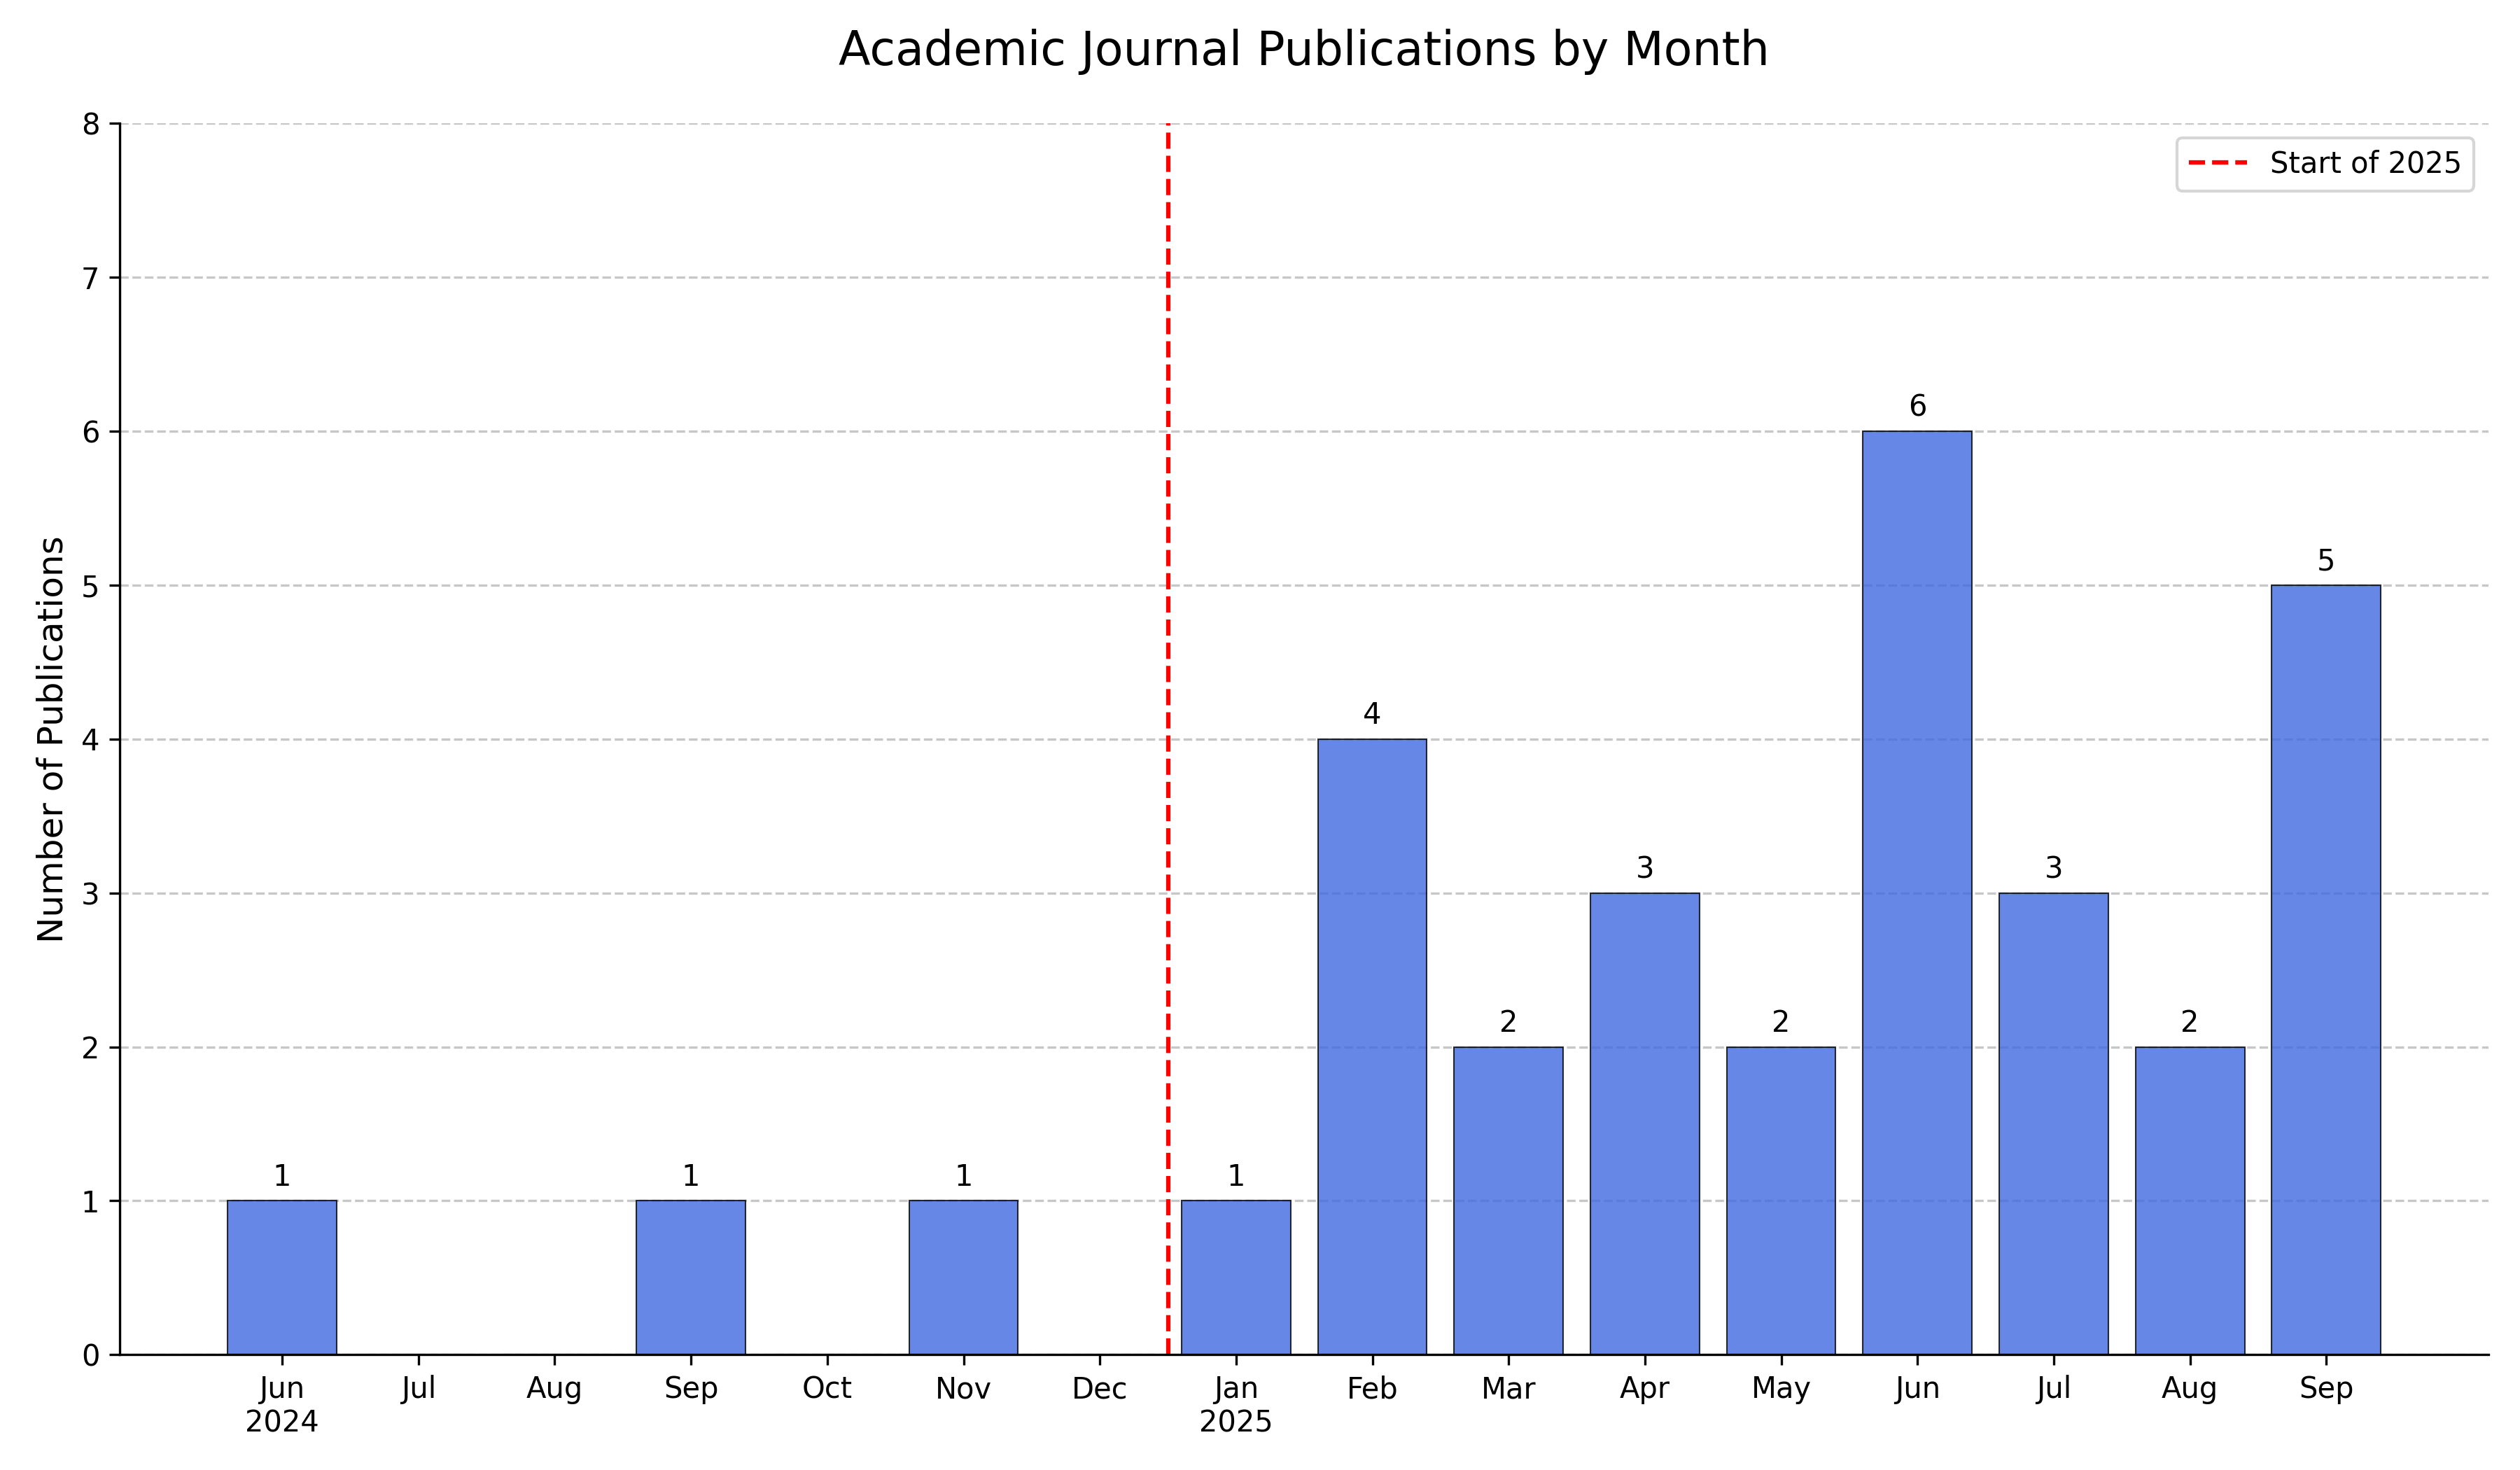
\includegraphics[width=0.9\linewidth]{./Images/monthly_publication_chart.png}
    \caption{Academic Journal Publications}
    \label{fig:monthly_publications}
\end{figure}



\section{Reporting the Review}

The third and last stage reports the analysis of the retained articles, research question by research question. The venue of every retained study is listed in \Cref{sec:appA_corpus}; the corpus is concentrated rather than diffuse, with ACM Transactions on Software Engineering and Methodology contributing ten and Information and Software Technology three, the remaining venues one each, consistent with a topic actively published across the field rather than owned by any single outlet.




\subsection{Benefits of AI and LLMs usage in Software Development}

The first research question concerns the benefits of AI and \ac{LLM} adoption for developers, companies and other stakeholders. \Cref{tab:benefits} collects those reported in the literature.

{\footnotesize
\begin{longtable}{>{\raggedright\arraybackslash} p{3cm} p{9.3cm} p{0.2cm} >{\raggedright\arraybackslash}p{1.8cm}}
\caption{Benefits of using AI and LLMs in Software Development}
\label{tab:benefits} \\

\toprule
\textbf{Benefits} & \textbf{Description} & \textbf{\#} & \textbf{References}\\
\midrule
\endfirsthead

\toprule
\textbf{Benefits} & \textbf{Description} & \textbf{\#} & \textbf{References}\\
\midrule
\endhead

\midrule
\multicolumn{4}{r}{\textit{Continued on next page}}\\
\bottomrule
\endfoot

\bottomrule
\endlastfoot

Improved Code Quality, Accuracy, and Traceability & "improving code quality and optimizing work with faster times" \cite{Farhanna:2025eu}. & 20 & \cite{Kim:2025is, Basha:2025tt, Gao:2025cc, Li:2025sc, Dong:2024sc, Jensen:2025me, Haque:2025la, Kim:2025ao, Qiu:2025ft, Farhanna:2025eu, Zhang:2025ea, Tkachuk:2025dc, Banh:2025cf, Bai:2025ci, Ahmed:2025ai, Ramos:2025aa, Jabrw:2025ss, Durrani:2024ad, Han:2025mg, Hemmat:2025rd} \\ \addlinespace

Increased Productivity and Efficiency & "converts natural language or abstract intent into functioning software modules, dramatically shortening development cycles" \cite{Moore:2025vc}. & 18 & \cite{Moore:2025vc, Basha:2025tt, Terragni:2025fa, Yoo:2025sa, Jensen:2025me, Haque:2025la, Kim:2025is, Qiu:2025ft, Farhanna:2025eu, Zamfiroiu:2025ec, Zhang:2025ea, Tkachuk:2025dc, Banh:2025cf, Kim:2025ao, Ahmed:2025ai, Ramos:2025aa, Chen:2025es, Wang:2025rs} \\ \addlinespace

Automation of Testing, Debugging, and Repair & AI and LLMs support "automating coding, bug detection, debugging, and personalizing software according to user needs" \cite{Farhanna:2025eu}. & 12 & \cite{Moore:2025vc, Terragni:2025fa, Gao:2025cc, Dong:2024sc, AlHashimi:2025er, Kim:2025ao, Ahmed:2025ai, Chen:2025es, Ramos:2025aa, Wang:2025rs, Kim:2025is, Qiu:2025ft} \\ \addlinespace

Optimization of Code Performance and Efficiency & "The proportionally small number of studies in SE subfields like Build, Release, Deploy, Operate and Monitor indicates a broad untapped area for cost savings and novelty" \cite{KarlovsKarlovskis:2024ga}. & 10 & \cite{Moore:2025vc, Terragni:2025fa, Haque:2025la, KarlovsKarlovskis:2024ga, Qiu:2025ft, Farhanna:2025eu, AlHashimi:2025er, Zamfiroiu:2025ec, Zhang:2025ea, Banh:2025cf} \\ \addlinespace

Support for Early Software Development Phases (Requirements \& Design) & AI and LLMs have effectiveness in "...enhancing stakeholder communication and requirement documentation" while noting challenges with bias and accuracy in requirements and design elicitation \cite{Kim:2025ao}. & 8 & \cite{Gao:2025cc, Terragni:2025fa, Hemmat:2025rd, Zhang:2025ea, Kim:2025ao, Durrani:2024ad, Jensen:2025me, Qiu:2025ft} \\ \addlinespace

Automated Documentation and Summarization & "LLMs can [...] automatically generate documentation for codebases [...] ensuring that documentation stays current and can be updated as code evolves" \cite{Haque:2025la}. & 8 & \cite{Terragni:2025fa, Haque:2025la, AlHashimi:2025er, Zhang:2025ea, Tkachuk:2025dc, Banh:2025cf, Jabrw:2025ss, Durrani:2024ad} \\ \addlinespace

Enhanced Security and Vulnerability Management & AI supports SDLC security through "vulnerability detection, threat modeling, secure coding practices, and incident response" \cite{AlHashimi:2025er}. & 6 & \cite{Terragni:2025fa, Yoo:2025sa, Qiu:2025ft, AlHashimi:2025er, Bai:2025ci, Jabrw:2025ss} \\ \addlinespace

Knowledge Acquisition and Understanding & "Reduce technical barriers and transform the programming process into a collaborative, conversational, and more accessible act" \cite{Zamfiroiu:2025ec}. & 5 & \cite{Zamfiroiu:2025ec, Banh:2025cf, Chen:2025es, Qiu:2025ft, Jensen:2025me} \\ \addlinespace

Management and Organizational Support & Assist in managing and "curating organizational information about day-to-day organizational practices" \cite{Jensen:2025me}. & 5 & \cite{Gao:2025cc, AlHashimi:2025er, Ahmed:2025ai, Durrani:2024ad, Zhang:2025ea} \\ \addlinespace

Developer Well-being and Satisfaction & "prioritize interesting and fun tasks through automating menial, boring tasks" \cite{Jensen:2025me}. & 4 & \cite{Jensen:2025me, Zhang:2025ea, Basha:2025tt, Qiu:2025ft} \\ \addlinespace

Democratization and Accessibility & "shift the programming paradigm from a traditional code-centric approach to one that involves verbal interactions between the programmer and the artificial intelligence agent" \cite{Zamfiroiu:2025ec}. & 2 & \cite{Zamfiroiu:2025ec, Moore:2025vc} \\ \addlinespace

\end{longtable}
}


The two most frequently reported benefits, productivity and code quality, are reported as mutually reinforcing: acceleration does not come at the cost of quality, since AI helps generate code adhering to high standards, raising the accuracy and traceability of the final product \cite{Kim:2025is}. Automating quality-assurance tasks, testing, debugging and repair supports the same synergy, and the mechanism is specific: LLMs leverage explicit feedback such as compiler error messages in follow-up prompts, iteratively fixing their own coding errors within a single conversation context. Beyond the codebase itself, the reported benefits extend to developer job satisfaction and to the democratisation of programming knowledge.

\subsection{Consequences of AI and LLMs usage in Software Development}

The second research question concerns the consequences that may arise from incorporating AI and \acp{LLM} into software development, in code generation and elsewhere. Those reported across the corpus are collected in \Cref{tab:consequences}.
{\footnotesize
\begin{longtable}{>{\raggedright\arraybackslash} p{3cm} p{9.3cm} p{0.2cm} >{\raggedright\arraybackslash}p{1.8cm}}
\caption{Consequences of using AI and LLMs in Software Development}
\label{tab:consequences} \\

\toprule
\textbf{Consequences} & \textbf{Description} & \textbf{\#} & \textbf{References}\\
\midrule
\endfirsthead

\toprule
\textbf{Consequences} & \textbf{Description} & \textbf{\#} & \textbf{References}\\
\midrule
\endhead

\midrule
\multicolumn{4}{r}{\textit{Continued on next page}}\\
\bottomrule
\endfoot

\bottomrule
\endlastfoot

Increased Operational Costs and Resource Constraints & "a substantial financial burden [...] when LLMs are deployed to handle a large number of tasks" \cite{Hou:2025cl}. & 20 & \cite{Terragni:2025fa, Han:2025mg, Haque:2025la, KarlovsKarlovskis:2024ga, Weyssow:2025ep, Hou:2025cl, Ahmed:2025ai, Chen:2025es, Jabrw:2025ss, Durrani:2024ad} \\ \addlinespace

Reliability, Accuracy, and Hallucination Risks & Particularly problematic in complex or niche scenarios: "this AI can simply make things up or sometimes spit out things that don’t even exist" \cite{Banh:2025cf}. & 15 & \cite{Basha:2025tt, Terragni:2025fa, Gao:2025cc, Li:2025sc, Hemmat:2025rd, Han:2025mg, Zamfiroiu:2025ec, Tkachuk:2025dc, Bai:2025ci, Chen:2025es, Durrani:2024ad, Zhang:2025ea, Kim:2025is, Ramos:2025aa, Wang:2025rs} \\ \addlinespace

Security Vulnerabilities in Generated Code & "AI-generated code may harbor unique security risks in areas such as cryptographic implementation, memory management, and error handling" \cite{Yoo:2025sa}. Existing tools do not close the gap: they detect only "46.7\% of vulnerabilities in AI-generated code, a significantly lower rate than for human-written code vulnerabilities (66.4\%)" \cite{Yoo:2025sa}. & 15 & \cite{Basha:2025tt, Gao:2025cc, Yoo:2025sa, KarlovsKarlovskis:2024ga, AlHashimi:2025er, Farhanna:2025eu, Tkachuk:2025dc, Banh:2025cf, Bai:2025ci, Ahmed:2025ai, Chen:2025es, Jabrw:2025ss, Haque:2025la, Qiu:2025ft, Wang:2025rs} \\ \addlinespace

Ethical, Legal, and Intellectual Property Issues & "questions about the ownership and licensing of that code will arise" when models are trained on publicly available, open-source projects \cite{Haque:2025la}. & 8 & \cite{Terragni:2025fa, AlHashimi:2025er, Zamfiroiu:2025ec, Ahmed:2025ai, Durrani:2024ad, Banh:2025cf, Basha:2025tt, Haque:2025la} \\ \addlinespace

Homogeneity and Bias Propagation & LLMs increasingly train on LLM-generated code, tending to "reaffirm patterns seen in their training data (e.g., public GitHub repositories)" \cite{Terragni:2025fa}. & 8 & \cite{Terragni:2025fa, Basha:2025tt, Haque:2025la, AlHashimi:2025er, Farhanna:2025eu, Banh:2025cf, Ahmed:2025ai, Ramos:2025aa} \\ \addlinespace

Evaluation and Standardization Challenges & "It is urgent to establish an effective, objective, and complete evaluation system for large language models for code" \cite{Ahmed:2025ai}. & 7 & \cite{Ahmed:2025ai, Yoo:2025sa, Hemmat:2025rd, Pendyala:2025pi, Farhanna:2025eu, Jabrw:2025ss, Han:2025mg} \\ \addlinespace

Risk of Over-reliance and Cognitive Decline & "if AI is constantly available, people will tend to become lazy and stop thinking for themselves" \cite{Banh:2025cf}. & 4 & \cite{Banh:2025cf, Basha:2025tt, Jensen:2025me, Zamfiroiu:2025ec} \\ \addlinespace

New Overhead and Workflow Inefficiencies (Human Review) & LLMs still "require human oversight and review of their outputs before implementation" \cite{Kim:2025ao}. & 4 & \cite{Kim:2025ao, Durrani:2024ad, Banh:2025cf, Zamfiroiu:2025ec} \\ \addlinespace

\end{longtable}
}


The consequences tabulated above are technical, ethical and operational, with
the technical and operational ones cited most often. Cost comes first:
training, fine-tuning and deploying large-scale models can be substantially
more expensive than traditional methods, offsetting the productivity gains
they are meant to buy. Reliability comes second: LLMs frequently produce
plausible but fabricated output, "hallucinations". The detection gap the
table records between AI-generated and human-written code is the same
problem from the tooling side, existing instruments being matched to failure
modes AI-generated code does not share \cite{Yoo:2025sa}.

Beyond the technical domain, adoption carries risks to human factors, ethics
and economic viability: over-reliance eroding developers' independence as
instant assistance becomes the default, training-data bias perpetuated and
magnified in generated code \cite{Haque:2025la}, and unresolved ownership and
licensing where models train on open-source code \cite{Terragni:2025fa}.

\subsection{Methodologies and management methods used to integrate AI and LLMs in Software Development}

The third research question asks which methodologies and management methods are used to integrate AI and \acp{LLM} into software development. \Cref{tab:methodologies} lists those the corpus reports.

{\footnotesize
\begin{longtable}{>{\raggedright\arraybackslash} p{3cm} p{9.3cm} p{0.2cm} >{\raggedright\arraybackslash}p{1.8cm}}
\caption[Methodologies and management methods for integrating AI and LLMs]{Methodologies and Management Methods used to integrate AI and LLMs in Software Development}
\label{tab:methodologies} \\

\toprule
\textbf{Methodologies} & \textbf{Description} & \textbf{\#} & \textbf{References}\\
\midrule
\endfirsthead

\toprule
\textbf{Methodologies} & \textbf{Description} & \textbf{\#} & \textbf{References}\\
\midrule
\endhead

\midrule
\multicolumn{4}{r}{\textit{Continued on next page}}\\
\bottomrule
\endfoot

\bottomrule
\endlastfoot

In-Context Learning (ICL) / Few-shot Learning & "integrating context-specific information, in the form of an input prompt or instruction template, during the inference and thus without the need to perform gradient-based training" \cite{Weyssow:2025ep}. & 9 & \cite{Weyssow:2025ep, Terragni:2025fa, Chen:2025es, Ramos:2025aa, Durrani:2024ad, Gao:2025cc, Hemmat:2025rd, Qiu:2025ft, Jabrw:2025ss} \\ \addlinespace

Prompt Engineering (PE) / Prompt-Driven Development & "The effectiveness of prompt engineering critically determines the performance of leveraging the capabilities of LLMs". \cite{Jabrw:2025ss} & 5 &  \cite{Jabrw:2025ss, Pendyala:2025pi, Qiu:2025ft, Ahmed:2025ai, Chen:2025es} \\ \addlinespace

Chain-of-Thought (CoT) Prompting & "A CoT is several intermediate natural language reasoning steps that lead to the final answer" \cite{Li:2025sc}. & 5 & \cite{Li:2025sc, Jabrw:2025ss, Chen:2025es, Ahmed:2025ai, Gao:2025cc} \\ \addlinespace

Human-In-The-Loop (HITL) Paradigm & "The importance of the human contribution in identifying and resolving problems to maintain software quality is widely acknowledged by many authors" \cite{Kim:2025ao}. \acp{LLM} still "require human oversight and review of their outputs before implementation" \cite{Kim:2025ao, Terragni:2025fa}. & 6 & \cite{Kim:2025ao, Wang:2025rs, Terragni:2025fa, Hemmat:2025rd, Haque:2025la, Zamfiroiu:2025ec}\\ \addlinespace

Structured Prompting / Structured Chain-of-Thought (SCoT) & "SCoT denotes several intermediate reasoning steps constructed by programming structures" \cite{Li:2025sc}. & 4 & \cite{Li:2025sc, Han:2025mg, Jabrw:2025ss, Kim:2025is} \\ \addlinespace

Multi-Agent Systems / Self-Collaboration Approach & "a self-collaboration framework with role instruction, which allows LLM agents to collaborate with each other to generate code for complex requirements" \cite{Wang:2025rs, Dong:2024sc}. & 4 & \cite{Wang:2025rs, Dong:2024sc, Banh:2025cf, Bai:2025ci} \\ \addlinespace

Integration with External Tools and Domain Knowledge & "Combining the linguistic capability of LLMs with specialized domain knowledge to enhance output quality, functionality, or security" \cite{Wang:2025rs, Banh:2025cf}. & 3 & \cite{Wang:2025rs, Banh:2025cf, Zhang:2025ea, Ahmed:2025ai} \\ \addlinespace

Other Single-Study Techniques & Five techniques each supported by a single study: Retrieval-Augmented Generation offers "a low-computation option by eliminating the need for parameter updates", though it "falls short of LoRA's effectiveness across all three CodeLlama model variants" \cite{Weyssow:2025ep, Chen:2025es}; AI-Augmented Agile Development (AgileGen) focuses human involvement on the start (scenario decision-making) and end (acceptance decision-making) of each iteration \cite{Zhang:2025ea}; Gherkin-based behaviour-driven testing supplements unclear user requirements with well-defined acceptance criteria \cite{Zhang:2025ea}; Vibe Coding converts natural language or abstract intent into functioning software modules \cite{Moore:2025vc}; and integrating LLMs with traditional testing approaches yields a "1.4× to 2.3× improvement than the baselines" \cite{Wang:2025rs}. & 5 & \cite{Weyssow:2025ep, Chen:2025es, Zhang:2025ea, Moore:2025vc, Wang:2025rs} \\ \addlinespace

\end{longtable}
}

The methods reported range from prompt-level tuning to large-scale process
frameworks, and they stratify into two tiers:

\begin{itemize}[leftmargin=0.6cm, itemsep=0.5em]
\item \textbf{Prompt-level tuning.} In-Context Learning (9 articles, the
most-discussed technique) and Prompt Engineering, whose quality critically
determines effectiveness, form the base layer. Chain-of-Thought and its
Structured variant apply the same principle, introducing programming
constructs such as sequence, branch and loop into the reasoning steps
\cite{Li:2025sc}.
\item \textbf{Process-level frameworks.} Given LLMs' variable reliability,
Human-In-The-Loop is considered mandatory for software quality
\cite{Kim:2025ao}: developers retain oversight, reviewing AI output before
implementation. AI-Augmented Agile Development (AgileGen) formalises this,
reserving human decision-making for the start (scenario definition) and end
(acceptance) of each iteration \cite{Zhang:2025ea}, preventing the error
accumulation unsupervised multi-agent systems risk.
\end{itemize}

"Vibe Coding", mentioned once in the corpus, is recent and not yet widely
studied \cite{Moore:2025vc}, but reliably translating a "vibe" into working
software is what the methodologies above exist to constrain.


\subsection{Developers' and other stakeholders' opinions regarding the use of AI and LLMs in Software Development}

The fourth research question concerns the human perspective. Reception differs enough between groups that the extracted opinions are tabulated separately in \Cref{sec:appA_opinions}, for the public and researchers, developers and practitioners, and organisations and management; the separation is itself a finding.

\begin{itemize}[leftmargin=0.6cm, itemsep=0.5em]
\item \textbf{Public and researchers.} Scepticism grounded in fallibility,
not capability, dominates. General perception (six articles) treats these
systems as a mixture of software and sorcery; the primary barrier reported
is misinformation risk, since generated code may execute without error
while failing the intended requirement, amplified by variability across
repeated identical prompts.
\item \textbf{Developers and practitioners.} The opposite emphasis:
productivity and efficiency gains are the most-cited positive opinion (six
articles), and \acp{LLM} are valued for knowledge acquisition, bypassing
extended search or dependence on colleagues~\cite{Banh:2025cf}. Two
countervailing findings appear alongside it: a documented risk of
over-reliance and skill erosion, and prompt design as a significant time
investment that reduces the efficiency it promises~\cite{Banh:2025cf}.
\item \textbf{Organisations and management.} Adoption is treated as a
risk-management exercise. The strategic case, retaining valuable staff by
automating routine work~\cite{Jensen:2025me}, is constrained by the
group's most-cited concern, data security and privacy (six articles). The
consensus strategy favours open models fine-tuned on organisation-specific
data over commercial \acp{LLM}, raising operational cost and pushing teams
towards medium-sized models; expectation management appears less often but
matters equally, discounting the hype
surrounding these tools when planning integration.
\end{itemize}

That is what makes the single most prevalent opinion across all three
groups, the need for human oversight with seven articles, follow from
evidence rather than from caution.

\subsection{Industry sectors adopting AI and LLMs for Software Applications Development}

The fifth research question asks which industry sectors are actively adopting \ac{AI} for application development and what sector-level benefits they report; the extracted evidence is tabulated in \Cref{sec:appA_sectors}.

Adoption concentrates overwhelmingly in Software Engineering, Software Development and IT Consulting, both the origin and the primary proving ground for \ac{LLM}-based tools. The reported use cases centre on code generation, completion, explanation and refactoring, and several sources describe a gradual shift in the developer role from writing code manually to orchestrating AI-enabled workflows in which the human directs, validates and refines automated output~\cite{Jensen:2025me, Zhang:2025ea, Kim:2025ao}. In consulting, \acp{LLM} are valued for accelerating onboarding and transferring client-specific business knowledge between projects; adoption also appears in infrastructure-level or mathematically intensive domains, where models must be adapted or augmented with structured knowledge to produce reliable output~\cite{Wang:2025rs, Hou:2025cl, Ahmed:2025ai, AlHashimi:2025er}.

Beyond the core \ac{IT} sector, adoption clusters in finance, banking and
regulated industries (eight articles), transportation and other
safety-critical domains (seven), healthcare and biomedical research (five),
education and training (five) and legal reasoning (four); education is an
emerging area in which \acp{LLM} act as adaptive learning companions rather
than replacements for educators, supporting exercise generation,
personalised feedback and formative
assessment~\cite{Ramos:2025aa, Hemmat:2025rd, Zamfiroiu:2025ec}.

In the first four, \acp{LLM} are introduced cautiously, with emphasis on
reliability, auditability and regulatory compliance, and the literature is
consistent that extensive human review remains mandatory wherever incorrect
or unverifiable output could produce safety risks, compliance failures or
legal liability~\cite{Moore:2025vc, Ahmed:2025ai, Jabrw:2025ss, Qiu:2025ft}.

No sector reports adopting these tools without a human check, and the sectors with the most to lose report the most explicit checks.

\section{Discussion}

Read across the five research questions, the review converges on a single
pattern. Every benefit reported under RQ1 has a
corresponding risk under RQ2 threatening the same property it claims: speed
and code quality against hallucination, security vulnerabilities and
homogenisation; democratised access against over-reliance and skill erosion.
The field's answer to that tension is not automation but control: every
prevalent method under RQ3, In-Context Learning, Prompt Engineering,
Chain-of-Thought and above all Human-In-The-Loop, exists to shape or
supervise AI output before it is trusted, and none proposes removing the
human; every stakeholder group under RQ4 pairs enthusiasm with a caveat,
human oversight being the one consensus surviving their differing
incentives; and under RQ5 it is the organising variable for adoption itself,
broad and unconditional where an incorrect output is cheap, explicitly
conditioned on verification where it is expensive, as in finance,
transportation or healthcare. The absence of a standardised, secure
integration methodology, not a shortfall in model capability, is therefore
what the literature identifies as the actual barrier to broader adoption,
the gap \Cref{chap:problem} formalises. \Cref{tab:ai_sdlc_mapping} restates
the pattern phase by phase; read down its challenge column and the same
requirement recurs at every one, a human check of the model's output against
something written before that output existed.

{\footnotesize
\begin{longtable}{p{2.3cm} p{11.5cm}}
\caption{Impact of AI and LLMs across Software Development Lifecycle Phases}
\label{tab:ai_sdlc_mapping} \\

\toprule
\textbf{SDLC Phase} & \textbf{Main Challenges} \\
\midrule
\endfirsthead

\toprule
\textbf{SDLC Phase} & \textbf{Main Challenges} \\
\midrule
\endhead

\midrule
\multicolumn{2}{r}{\textit{Continued on next page}}\\
\bottomrule
\endfoot

\bottomrule
\endlastfoot

Requirements Analysis &
Risk of ambiguity amplification, overconfidence in AI-generated requirements, and lack of domain context; increased need for human validation early in the process. \\
\addlinespace

Design &
Limited understanding of system-wide constraints; risk of inconsistent or suboptimal architectural decisions without expert oversight. \\
\addlinespace

Implementation &
Hallucinated code, inconsistent outputs, security vulnerabilities, and reduced trust due to output variability; heavy reliance on human review. \\
\addlinespace

Testing &
Difficulty validating correctness of AI-generated tests; increased testing complexity due to unpredictable AI-generated code. \\
\addlinespace

Deployment &
Risk of misconfiguration or insecure defaults; limited contextual awareness of operational environments. \\
\addlinespace

Maintenance &
Potential over-reliance on AI explanations; challenges in maintaining long-term system understanding and accountability. \\
\addlinespace

\end{longtable}
}




